


%\tikzset{every picture/.style={line width=0.75pt}} %set default line width to 0.75pt        


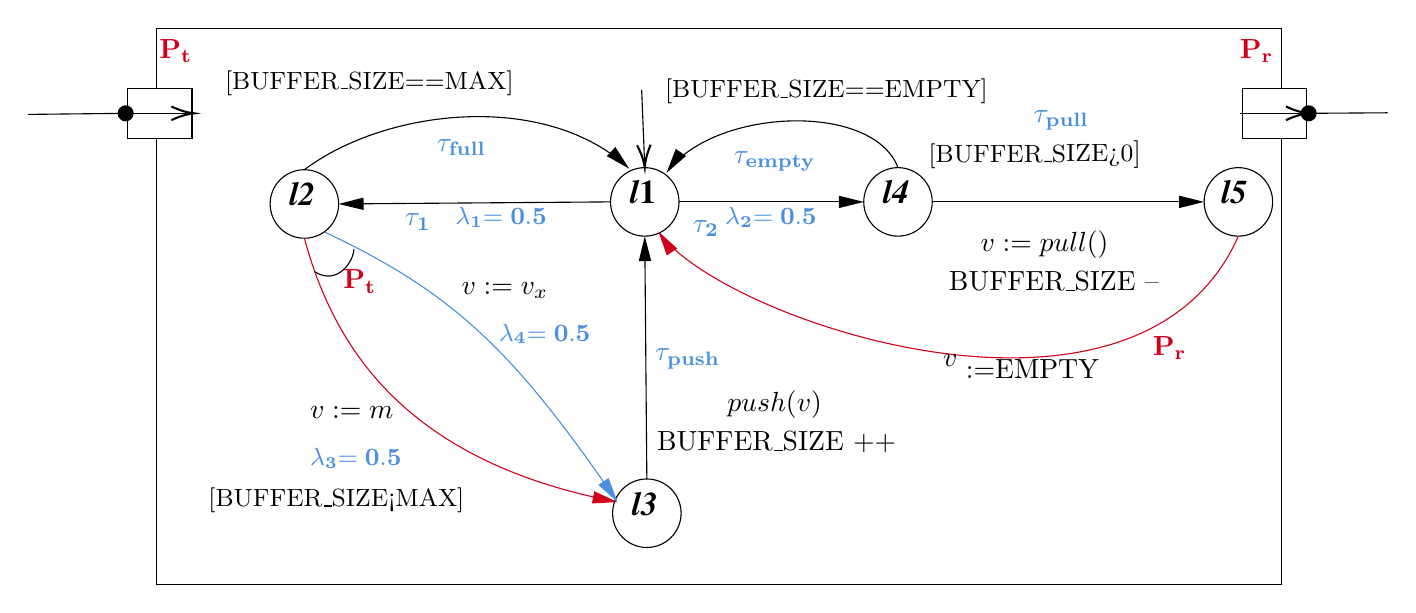
\begin{tikzpicture}[x=0.75pt,y=0.75pt,yscale=-1,xscale=1]
%uncomment if require: \path (0,300); %set diagram left start at 0, and has height of 300

%Shape: Ellipse [id:dp010084959855120812] 
\draw   (272,94.5) .. controls (272,85.39) and (279.39,78) .. (288.5,78) .. controls (297.61,78) and (305,85.39) .. (305,94.5) .. controls (305,103.61) and (297.61,111) .. (288.5,111) .. controls (279.39,111) and (272,103.61) .. (272,94.5) -- cycle ;
%Shape: Ellipse [id:dp49635434136123957] 
\draw   (108,95.5) .. controls (108,86.39) and (115.39,79) .. (124.5,79) .. controls (133.61,79) and (141,86.39) .. (141,95.5) .. controls (141,104.61) and (133.61,112) .. (124.5,112) .. controls (115.39,112) and (108,104.61) .. (108,95.5) -- cycle ;
%Shape: Ellipse [id:dp6951277589405004] 
\draw   (394,94.5) .. controls (394,85.39) and (401.39,78) .. (410.5,78) .. controls (419.61,78) and (427,85.39) .. (427,94.5) .. controls (427,103.61) and (419.61,111) .. (410.5,111) .. controls (401.39,111) and (394,103.61) .. (394,94.5) -- cycle ;
%Shape: Ellipse [id:dp20139765197933113] 
\draw   (558,94.5) .. controls (558,85.39) and (565.39,78) .. (574.5,78) .. controls (583.61,78) and (591,85.39) .. (591,94.5) .. controls (591,103.61) and (583.61,111) .. (574.5,111) .. controls (565.39,111) and (558,103.61) .. (558,94.5) -- cycle ;
%Shape: Ellipse [id:dp8470834514834077] 
\draw   (273,244.5) .. controls (273,235.39) and (280.39,228) .. (289.5,228) .. controls (298.61,228) and (306,235.39) .. (306,244.5) .. controls (306,253.61) and (298.61,261) .. (289.5,261) .. controls (280.39,261) and (273,253.61) .. (273,244.5) -- cycle ;
%Straight Lines [id:da6289943518790769] 
\draw    (272,94.5) -- (143,95.48) ;
\draw [shift={(141,95.5)}, rotate = 359.56] [fill={rgb, 255:red, 0; green, 0; blue, 0 }  ][line width=0.08]  [draw opacity=0] (12,-3) -- (0,0) -- (12,3) -- cycle    ;
%Straight Lines [id:da5157806883764975] 
\draw    (305,94.5) -- (392,94.5) ;
\draw [shift={(394,94.5)}, rotate = 180] [fill={rgb, 255:red, 0; green, 0; blue, 0 }  ][line width=0.08]  [draw opacity=0] (12,-3) -- (0,0) -- (12,3) -- cycle    ;
%Curve Lines [id:da8099696982957123] 
\draw    (124.5,79) .. controls (164.1,49.3) and (239.96,41.33) .. (279.8,77.39) ;
\draw [shift={(281,78.5)}, rotate = 223.38] [fill={rgb, 255:red, 0; green, 0; blue, 0 }  ][line width=0.08]  [draw opacity=0] (12,-3) -- (0,0) -- (12,3) -- cycle    ;
%Curve Lines [id:da3041106263261554] 
\draw    (410.5,78) .. controls (398.55,46.32) and (323.18,49.24) .. (300.02,79.12) ;
\draw [shift={(299,80.5)}, rotate = 305.05] [fill={rgb, 255:red, 0; green, 0; blue, 0 }  ][line width=0.08]  [draw opacity=0] (12,-3) -- (0,0) -- (12,3) -- cycle    ;
%Straight Lines [id:da8355039005427021] 
\draw    (427,94.5) -- (556,94.5) ;
\draw [shift={(558,94.5)}, rotate = 180] [fill={rgb, 255:red, 0; green, 0; blue, 0 }  ][line width=0.08]  [draw opacity=0] (12,-3) -- (0,0) -- (12,3) -- cycle    ;
%Straight Lines [id:da6140071615749851] 
\draw    (289.5,228) -- (288.52,113) ;
\draw [shift={(288.5,111)}, rotate = 89.51] [fill={rgb, 255:red, 0; green, 0; blue, 0 }  ][line width=0.08]  [draw opacity=0] (12,-3) -- (0,0) -- (12,3) -- cycle    ;
%Curve Lines [id:da053683210347318044] 
\draw [color={rgb, 255:red, 208; green, 2; blue, 27 }  ,draw opacity=1 ]   (574.5,111) .. controls (526.49,219.57) and (327.04,152.05) .. (295.89,109.93) ;
\draw [shift={(295,108.67)}, rotate = 56.31] [fill={rgb, 255:red, 208; green, 2; blue, 27 }  ,fill opacity=1 ][line width=0.08]  [draw opacity=0] (12,-3) -- (0,0) -- (12,3) -- cycle    ;
%Curve Lines [id:da3918683875841986] 
\draw [color={rgb, 255:red, 208; green, 2; blue, 27 }  ,draw opacity=1 ]   (124.5,112) .. controls (139.29,166.82) and (175.01,219.57) .. (273.87,238.81) ;
\draw [shift={(275.37,239.1)}, rotate = 190.76] [fill={rgb, 255:red, 208; green, 2; blue, 27 }  ,fill opacity=1 ][line width=0.08]  [draw opacity=0] (12,-3) -- (0,0) -- (12,3) -- cycle    ;
%Shape: Rectangle [id:dp3826164922815618] 
\draw   (53.37,10.83) -- (595.37,10.83) -- (595.37,278.83) -- (53.37,278.83) -- cycle ;
%Shape: Rectangle [id:dp24979110898438062] 
\draw  [fill={rgb, 255:red, 255; green, 255; blue, 255 }  ,fill opacity=1 ] (39.37,39.92) -- (70.37,39.92) -- (70.37,63.75) -- (39.37,63.75) -- cycle ;
%Straight Lines [id:da5999486284548592] 
\draw    (38.37,51.83) -- (69.37,51.83) ;
\draw [shift={(71.37,51.83)}, rotate = 180] [color={rgb, 255:red, 0; green, 0; blue, 0 }  ][line width=0.75]    (10.93,-3.29) .. controls (6.95,-1.4) and (3.31,-0.3) .. (0,0) .. controls (3.31,0.3) and (6.95,1.4) .. (10.93,3.29)   ;
%Straight Lines [id:da6692676292533337] 
\draw    (-8.55,52.35) -- (38.37,51.83) ;
\draw [shift={(38.37,51.83)}, rotate = 359.37] [color={rgb, 255:red, 0; green, 0; blue, 0 }  ][fill={rgb, 255:red, 0; green, 0; blue, 0 }  ][line width=0.75]      (0, 0) circle [x radius= 3.35, y radius= 3.35]   ;

%Shape: Rectangle [id:dp9523101657403588] 
\draw  [fill={rgb, 255:red, 255; green, 255; blue, 255 }  ,fill opacity=1 ] (576.37,39.92) -- (607.37,39.92) -- (607.37,63.75) -- (576.37,63.75) -- cycle ;
%Straight Lines [id:da13014540149939957] 
\draw    (575.37,51.83) -- (606.37,51.83) ;
\draw [shift={(608.37,51.83)}, rotate = 180] [color={rgb, 255:red, 0; green, 0; blue, 0 }  ][line width=0.75]    (10.93,-3.29) .. controls (6.95,-1.4) and (3.31,-0.3) .. (0,0) .. controls (3.31,0.3) and (6.95,1.4) .. (10.93,3.29)   ;
%Curve Lines [id:da7958000429185483] 
\draw [color={rgb, 255:red, 74; green, 144; blue, 226 }  ,draw opacity=1 ]   (134.37,109.1) .. controls (195.92,138.05) and (225.07,165.82) .. (274.62,238.01) ;
\draw [shift={(275.37,239.1)}, rotate = 235.59] [fill={rgb, 255:red, 74; green, 144; blue, 226 }  ,fill opacity=1 ][line width=0.08]  [draw opacity=0] (12,-3) -- (0,0) -- (12,3) -- cycle    ;
%Curve Lines [id:da4303220634916789] 
\draw    (129.37,128.1) .. controls (140.37,135.1) and (148.37,123.1) .. (148.37,117.1) ;
%Straight Lines [id:da23361338797732878] 
\draw    (608.37,51.83) -- (646.37,51.57) ;
\draw [shift={(608.37,51.83)}, rotate = 359.6] [color={rgb, 255:red, 0; green, 0; blue, 0 }  ][fill={rgb, 255:red, 0; green, 0; blue, 0 }  ][line width=0.75]      (0, 0) circle [x radius= 3.35, y radius= 3.35]   ;
%Straight Lines [id:da1676112371160593] 
\draw    (287,40.5) -- (288.42,76) ;
\draw [shift={(288.5,78)}, rotate = 267.71] [color={rgb, 255:red, 0; green, 0; blue, 0 }  ][line width=0.75]    (10.93,-3.29) .. controls (6.95,-1.4) and (3.31,-0.3) .. (0,0) .. controls (3.31,0.3) and (6.95,1.4) .. (10.93,3.29)   ;


% Text Node
\draw (431,167) node [anchor=north west][inner sep=0.75pt]    {$v$};
% Text Node
\draw (327,184) node [anchor=north west][inner sep=0.75pt]    {$push( v)$};
% Text Node
\draw (449,107) node [anchor=north west][inner sep=0.75pt]    {$v:=pull()$};
% Text Node
\draw (126,192) node [anchor=north west][inner sep=0.75pt]    {$v:=m$};
% Text Node
\draw (199,132) node [anchor=north west][inner sep=0.75pt]    {$v:=v_{x}$};
% Text Node
\draw (217,152) node [anchor=north west][inner sep=0.75pt]  [font=\small]  {$\mathbf{\textcolor[rgb]{0.29,0.56,0.89}{\lambda }\textcolor[rgb]{0.29,0.56,0.89}{_{4}}\textcolor[rgb]{0.29,0.56,0.89}{=0.5}}$};
% Text Node
\draw (126,212) node [anchor=north west][inner sep=0.75pt]  [font=\small]  {$\mathbf{\textcolor[rgb]{0.29,0.56,0.89}{\lambda }\textcolor[rgb]{0.29,0.56,0.89}{_{3}}\textcolor[rgb]{0.29,0.56,0.89}{=0.5}}$};
% Text Node
\draw (430,127) node [anchor=north west][inner sep=0.75pt]   [align=left] {\begin{minipage}[lt]{81.5pt}\setlength\topsep{0pt}
\begin{center}
BUFFER\_SIZE --
\end{center}

\end{minipage}};
% Text Node
\draw (565,83) node [anchor=north west][inner sep=0.75pt]   [align=left] {\textit{{\fontfamily{ptm}\selectfont \textbf{{\large l5}}}}};
% Text Node
\draw (116,84) node [anchor=north west][inner sep=0.75pt]   [align=left] {\textit{{\fontfamily{ptm}\selectfont \textbf{{\large l2}}}}};
% Text Node
\draw (281,233) node [anchor=north west][inner sep=0.75pt]   [align=left] {\textit{{\fontfamily{ptm}\selectfont \textbf{{\large l3}}}}};
% Text Node
\draw (280,83) node [anchor=north west][inner sep=0.75pt]   [align=left] {{\fontfamily{ptm}\selectfont \textbf{{\large \textit{l}1}}}};
% Text Node
\draw (402,83) node [anchor=north west][inner sep=0.75pt]   [align=left] {\textit{{\fontfamily{ptm}\selectfont \textbf{{\large l4}}}}};
% Text Node
\draw (77,231) node [anchor=north west][inner sep=0.75pt]  [font=\small] [align=left] {[BUFFER\_SIZE<MAX]};
% Text Node
\draw (574,15) node [anchor=north west][inner sep=0.75pt]  [color={rgb, 255:red, 208; green, 2; blue, 27 }  ,opacity=1 ]  {$\mathbf{P_{r}}$};
% Text Node
\draw (532,158) node [anchor=north west][inner sep=0.75pt]  [color={rgb, 255:red, 208; green, 2; blue, 27 }  ,opacity=1 ]  {$\mathbf{P_{r}}$};
% Text Node
\draw (142,126) node [anchor=north west][inner sep=0.75pt]  [color={rgb, 255:red, 208; green, 2; blue, 27 }  ,opacity=1 ]  {$\mathbf{P_{t}}$};
% Text Node
\draw (442,169) node [anchor=north west][inner sep=0.75pt]   [align=left] {:=EMPTY};
% Text Node
\draw (309.14,170.19) node  [color={rgb, 255:red, 74; green, 144; blue, 226 }  ,opacity=1 ]  {$\mathbf{\tau _{push}}$};
% Text Node
\draw (293,204) node [anchor=north west][inner sep=0.75pt]   [align=left] {\begin{minipage}[lt]{86.62pt}\setlength\topsep{0pt}
\begin{center}
BUFFER\_SIZE ++
\end{center}

\end{minipage}};
% Text Node
\draw (423.95,64.28) node [anchor=north west][inner sep=0.75pt]  [rotate=-359.76] [align=left] {{\small [BUFFER\_SIZE>0}]};
% Text Node
\draw (489.14,55.19) node  [color={rgb, 255:red, 74; green, 144; blue, 226 }  ,opacity=1 ]  {$\mathbf{\tau _{pull}}$};
% Text Node
\draw (297,34) node [anchor=north west][inner sep=0.75pt]  [font=\small] [align=left] {[BUFFER\_SIZE==EMPTY]};
% Text Node
\draw (351.14,75.19) node  [color={rgb, 255:red, 74; green, 144; blue, 226 }  ,opacity=1 ]  {$\mathbf{\tau _{empty}}$};
% Text Node
\draw (200.14,68.19) node  [color={rgb, 255:red, 74; green, 144; blue, 226 }  ,opacity=1 ]  {$\mathbf{\tau _{full}}$};
% Text Node
\draw (85,30) node [anchor=north west][inner sep=0.75pt]  [font=\small] [align=left] {[BUFFER\_SIZE==MAX]};
% Text Node
\draw (326,96) node [anchor=north west][inner sep=0.75pt]  [font=\small]  {$\mathbf{\textcolor[rgb]{0.29,0.56,0.89}{\lambda }\textcolor[rgb]{0.29,0.56,0.89}{_{2}}\textcolor[rgb]{0.29,0.56,0.89}{=0.5}}$};
% Text Node
\draw (317.99,107.19) node  [color={rgb, 255:red, 74; green, 144; blue, 226 }  ,opacity=1 ]  {$\mathbf{\tau _{2}}$};
% Text Node
\draw (196,96) node [anchor=north west][inner sep=0.75pt]  [font=\small]  {$\mathbf{\textcolor[rgb]{0.29,0.56,0.89}{\lambda }\textcolor[rgb]{0.29,0.56,0.89}{_{1}}\textcolor[rgb]{0.29,0.56,0.89}{=0.5}}$};
% Text Node
\draw (179.14,104.19) node  [color={rgb, 255:red, 74; green, 144; blue, 226 }  ,opacity=1 ]  {$\mathbf{\tau _{1}}$};
% Text Node
\draw (53.37,14.83) node [anchor=north west][inner sep=0.75pt]  [color={rgb, 255:red, 208; green, 2; blue, 27 }  ,opacity=1 ]  {$\mathbf{P_{t}}$};


\end{tikzpicture}
